% !TeX program = pdflatex
%==============================================================================
%  Aula 07 --- Classificação e Classificadores Gaussianos
%  VERSÃO DO ALUNO: texto para leitura autônoma, fora da sala.
%  (O roteiro de sala é "07 Classificacao e Classificadores Gaussianos.tex".)
%==============================================================================
\documentclass[11pt,a4paper]{article}
\usepackage[aluno]{../../recursos/latex/estilo-notas}

\title{}
\date{}

\begin{document}
\cabecalhoaula{07}{Classificação e Classificadores Gaussianos}{AME §7.1--7.3 e §8.1; ISLP §2.2.3, §4.3 e §4.4}

%==============================================================================
\section*{O que você vai aprender}
%==============================================================================
Ao final desta aula você deve ser capaz de:
\begin{itemize}[leftmargin=1.4cm]
  \item formular o problema de classificação com a \emph{perda 0--1} e derivar o
        \textbf{classificador de Bayes};
  \item descrever a estratégia \emph{plug-in}: estimar $\Prob(Y=c\mid\x)$ e
        classificar pela maior probabilidade;
  \item estimar essa probabilidade pelo Teorema de Bayes, com o \textbf{Bayes
        ingênuo} (covariáveis contínuas ou discretas) e com a \textbf{análise
        discriminante} (LDA e QDA);
  \item entender por que LDA tem fronteira \emph{linear} e QDA \emph{quadrática};
  \item escolher entre LDA e QDA pelo balanço viés--variância;
  \item estimá-la diretamente, com uma \textbf{regressão logística} ajustada por
        máxima verossimilhança, e reconhecer sua versão penalizada e a multiclasse;
  \item contrastar as abordagens \emph{generativa} e \emph{discriminativa}.
\end{itemize}

\noindent
Começa aqui o Bloco~II, e a boa notícia é que \emph{quase tudo} do Bloco~I se
transfere: risco, balanço viés--variância, validação cruzada, \emph{pipelines}. A
única mudança é que $Y$ agora é \emph{qualitativo}, e por isso a perda natural
deixa de ser a quadrática e passa a ser a 0--1. Comece pela pergunta:

\begin{center}\itshape
  qual é o melhor classificador possível, se eu conhecesse\\
  a distribuição dos dados?
\end{center}

\noindent
Essa pergunta tem resposta exata e curta --- Teorema~\ref{teo:bayes} --- e ela
desempenha, aqui, exatamente o papel que $r(\x)=\E[Y\mid\X=\x]$ desempenhou na
Aula~01: define o alvo que todo método vai tentar aproximar.

%==============================================================================
\section{O problema de classificação}
%==============================================================================
Agora $Y$ assume valores num conjunto finito de \textbf{classes} $\mathcal{C}$ (ex.:
$\mathcal{C}=\{0,1\}$ no caso binário). Um \textbf{classificador} é uma função
$g:\R^p\to\mathcal{C}$, e queremos, como em regressão, que ela acerte observações
novas: $g(\x_{n+1})\approx y_{n+1}$.

O primeiro passo é decidir o que esse ``$\approx$'' quer dizer. A perda quadrática
$(Y-g(\X))^2$ não serve: se $Y$ é ``\emph{spam}'' ou ``não \emph{spam}'', não existe
a diferença $Y-g(\X)$. Codificar as classes por números não resolve, porque a conta
passa a depender de uma escolha arbitrária --- com três classes codificadas como
$1$, $2$ e $3$, confundir a classe~1 com a~3 custaria $4$, e com a~2 custaria $1$,
como se houvesse uma ordem entre as classes. Em classificação só há duas
situações: $g(\x)=y$, um acerto, e $g(\x)\ne y$, um erro. A perda que registra
exatamente isso é a \textbf{perda 0--1}, $L(y,g(\x))=\1{y\ne g(\x)}$, e o risco
correspondente é a \emph{probabilidade de erro}:
\begin{equation}\label{eq:risco01}
  \risco(g) = \E\big[\1{Y\ne g(\X)}\big] = \Prob\big(Y\ne g(\X)\big).
\end{equation}

\begin{teorema}[Classificador de Bayes]\label{teo:bayes}
Sob a perda 0--1, o classificador que minimiza \eqref{eq:risco01} é
\[
  g^*(\x) = \argmax_{c\in\mathcal{C}}\ \Prob(Y=c\mid \X=\x).
\]
No caso binário $\mathcal{C}=\{0,1\}$: $g^*(\x)=1 \iff \Prob(Y=1\mid\x)\ge \tfrac12$.
\end{teorema}
\begin{proof}
(Caso binário, classes $c_1,c_2$.) Condicionando em $\X$,
\[
  \risco(g)=\Prob(Y\ne g(\X))
  =\int \big[\1{g(\x)=c_2}\Prob(Y=c_1\mid\x)+\1{g(\x)=c_1}\Prob(Y=c_2\mid\x)\big]f(\x)\,d\x.
\]
Para \emph{cada} $\x$, o integrando é minimizado escolhendo $g(\x)=c_1$ quando
$\Prob(Y=c_1\mid\x)\ge\Prob(Y=c_2\mid\x)$ e $g(\x)=c_2$ caso contrário --- isto é,
a classe de maior probabilidade a posteriori. Como cada $\x$ é otimizado
pontualmente, o classificador resultante minimiza o risco global.
\end{proof}

\begin{ideia}
Note o padrão: como na Aula~01, em que se mostrou que $r$ minimiza o erro quadrático
esperado, a prova otimiza \emph{ponto a ponto} e depois integra. É a mesma técnica
--- e é por isso que os dois resultados se parecem tanto. Em regressão, o alvo é a
\emph{média} condicional; em classificação, a \emph{moda} condicional. O
classificador de Bayes $g^*$ é o ``oráculo'': nenhum classificador faz melhor. Seu
risco $R^*$ é o análogo do \emph{erro irredutível}. Mas $g^*$ é
\emph{desconhecido}, pois depende de $\Prob(Y=c\mid\x)$. Todo método desta aula é
uma tentativa de aproximá-lo.
\end{ideia}

\begin{observacao}[O que se transfere da Parte~I]
A estimação do risco \eqref{eq:risco01} é feita por \emph{data splitting}/validação
cruzada (Aula~03), agora medindo a \emph{proporção de erros} na validação. O balanço
viés--variância também vale: $R(g)-R^*$ decompõe-se num termo tipo variância (classe
$\mathcal{G}$ grande demais) e num termo tipo viés (classe pequena demais). E, como
em regressão, compare \emph{poucos} modelos no teste --- faça o \emph{tuning} por CV
dentro do treino.
\end{observacao}

\begin{atencao}
A acurácia (1 $-$ risco 0--1) pode \textbf{enganar} em dados desbalanceados: com 10
doentes em 1000, o classificador trivial ``todos saudáveis'' acerta 99\% --- e é
inútil. Precisaremos de outras métricas (matriz de confusão, sensibilidade,
precisão) --- tema da Aula~08.
\end{atencao}

%==============================================================================
\section{Classificadores \emph{plug-in}}
%==============================================================================
O Teorema~\ref{teo:bayes} sugere uma receita direta, dita \textbf{\emph{plug-in}}:
\begin{enumerate}[leftmargin=1.6cm,nosep]
  \item estime $\widehat\Prob(Y=c\mid\x)$ para cada classe $c\in\mathcal{C}$;
  \item classifique $\ghat(\x)=\argmax_{c\in\mathcal{C}}\widehat\Prob(Y=c\mid\x)$.
\end{enumerate}
Os métodos diferem em \emph{como} estimam $\Prob(Y=c\mid\x)$. Há duas grandes
famílias:
\begin{description}[leftmargin=2.6cm,style=nextline]
  \item[Generativos] modelam $f(\x\mid Y=c)$ e $\Prob(Y=c)$ e invertem com o
        Teorema de Bayes --- é o caso do Bayes ingênuo, do LDA e do QDA, as
        próximas seções.
  \item[Discriminativos] modelam $\Prob(Y=c\mid\x)$ \emph{diretamente} --- é o caso
        da regressão logística, que fecha a aula.
\end{description}

%==============================================================================
\section{Modelos generativos: o Teorema de Bayes}
%==============================================================================
A primeira família não modela $\Prob(Y=c\mid\x)$ diretamente; modela como os dados de
cada classe são gerados, e inverte:
\begin{equation}\label{eq:gen}
  \Prob(Y=c\mid\x) = \frac{f(\x\mid Y=c)\,\Prob(Y=c)}
                          {\sum_{s\in\mathcal{C}} f(\x\mid Y=s)\,\Prob(Y=s)},
\end{equation}
em que $f(\x\mid Y=c)$ é a densidade de $\X$ dentro da classe $c$ --- ou a função de
probabilidade, se $\X$ for discreto. Estima-se $\Prob(Y=c)$ pelas \emph{proporções
amostrais} de cada classe e $f(\x\mid Y=c)$ por algum modelo. Como o denominador de
\eqref{eq:gen} é o mesmo para todas as classes, basta comparar os numeradores:
\[
  \ghat(\x) = \argmax_{c\in\mathcal{C}}\ \widehat f(\x\mid Y=c)\,\widehat\Prob(Y=c).
\]
Os métodos das duas próximas seções se distinguem pelo modelo de $f(\x\mid Y=c)$.

\begin{ideia}[a inversão que dá nome à família]
Repare no que \eqref{eq:gen} pede. Em vez de perguntar ``dado este $\x$, qual a
classe?'', pergunta-se ``\emph{se} a classe fosse $c$, que $\x$ eu esperaria ver?''
--- e o Teorema de Bayes inverte a resposta. Daí o nome \emph{generativo}: o modelo
descreve como os dados são \textbf{gerados}, e por isso permite \emph{simular}
observações novas de cada classe, coisa que um modelo discriminativo, como a
regressão logística do fim da aula, não faz.
\end{ideia}

%==============================================================================
\section{Bayes ingênuo}
%==============================================================================
O Bayes ingênuo supõe \textbf{independência condicional} das covariáveis dada a
classe:
\begin{equation}\label{eq:nb}
  f(\x\mid Y=c) = \prod_{j=1}^p f(x_j\mid Y=c).
\end{equation}
É a hipótese ``ingênua'' que dá nome ao método: dentro de cada classe, as
componentes de $\X$ são tratadas como independentes. Ela quase nunca é literalmente
verdadeira, mas é \emph{conveniente} e frequentemente gera bons classificadores. A
conveniência é enorme: em vez de estimar uma densidade em $\R^p$ --- tarefa
condenada pela maldição da dimensionalidade --- estimam-se $p$ densidades em $\R^1$.
É a esparsidade de suposições comprando viabilidade.

\subsection{Covariáveis contínuas}
Cada $f(x_j\mid Y=c)$ pode ser \emph{qualquer} densidade em $\R$, e escolhê-la é um
problema de inferência univariada, resolvido só com as observações da covariável $j$
que pertencem à classe $c$. Por isso vale olhar os dados antes: um histograma por
classe mostra se a normal é razoável, se a variável é positiva e assimétrica, se há
caudas pesadas --- e ter à mão um bom repertório de modelos probabilísticos paga
aqui. Se nenhum modelo paramétrico servir, cada $f(x_j\mid Y=c)$ pode ser estimada
de forma não paramétrica.

A escolha mais comum é a gaussiana, $X_j\mid Y=c \sim N(\mu_{j,c},\sigma^2_{j,c})$,
com os estimadores de máxima verossimilhança
\[
  \widehat\mu_{j,c} = \frac{1}{\abs{\mathcal{C}_c}}\sum_{i\in\mathcal{C}_c} x_{i,j},
  \qquad
  \widehat\sigma^2_{j,c} = \frac{1}{\abs{\mathcal{C}_c}}\sum_{i\in\mathcal{C}_c}
    \big(x_{i,j}-\widehat\mu_{j,c}\big)^2,
\]
em que $\mathcal{C}_c=\{i: y_i=c\}$ reúne as observações de treino da classe $c$.
É o que faz o \texttt{GaussianNB} do \texttt{scikit-learn}, que ainda soma às
variâncias um termo minúsculo, para estabilidade numérica.

\subsection{Covariáveis discretas}
Se $\X$ é discreto, \eqref{eq:gen} vale com probabilidades no lugar das densidades, e
a hipótese ingênua fatora
$\Prob(\X=\x\mid Y=c)=\prod_{j=1}^p\Prob(X_j=x_j\mid Y=c)$. A estimação é análoga:
proporções calculadas dentro de cada classe. O \texttt{scikit-learn} traz as
variantes mais comuns:
\begin{itemize}[leftmargin=1.4cm,nosep]
  \item \texttt{BernoulliNB}: cada $X_j$ é binária,
        $X_j\mid Y=c\sim\text{Bernoulli}(\theta_{j,c})$;
  \item \texttt{CategoricalNB}: cada $X_j$ é categórica, com uma probabilidade por
        nível e por classe;
  \item \texttt{MultinomialNB}: $\X$ é um vetor de contagens --- quantas vezes cada
        palavra aparece num texto, por exemplo --- modelado por uma multinomial;
  \item \texttt{ComplementNB}: uma variante do multinomial, pensada para classes
        desbalanceadas.
\end{itemize}
O caso multinomial merece uma observação. As contagens de uma multinomial
\emph{não} são independentes entre si --- elas somam o tamanho do texto ---, mas a
hipótese ingênua continua lá, agora sobre as palavras: dada a classe, cada palavra
do texto é sorteada independentemente das outras. É a versão que funciona tão bem em
texto, e ela reaparece na Aula~E3.

\begin{atencao}
Numericamente, o produto \eqref{eq:nb} de muitos termos pequenos sofre
\emph{underflow} (vira $0$). Trabalhe sempre em \textbf{escala logarítmica}:
$\ghat(\x)=\argmax_c\big[\sum_j \log \widehat f(x_j\mid Y=c)+\log\widehat\Prob(Y=c)\big]$.
\end{atencao}

\begin{atencao}[o preço do ``ingênuo'']
Quando as covariáveis são de fato correlacionadas, o Bayes ingênuo conta a mesma
evidência várias vezes --- se três colunas dizem quase a mesma coisa, ele as trata
como três testemunhas independentes. O efeito é curioso e importante: a
\emph{ordenação} das observações costuma sair boa (ele acerta quem é mais provável
de ser da classe~1), mas as \emph{probabilidades} saem grudadas em $0$ e $1$. A
Aula~08 mede isso.
\end{atencao}

%==============================================================================
\section{Análise discriminante: LDA e QDA}
%==============================================================================
A análise discriminante abandona a independência: modela o vetor $\X$ inteiro,
dentro de cada classe, como \textbf{gaussiano multivariado}. Lembre que
$\bm{Z}\sim N(\bm{\mu},\bm{\Sigma})$ em $\R^p$ tem densidade
\begin{equation}\label{eq:normal}
  f(\bm{z}) = \frac{1}{\sqrt{(2\pi)^p\det\bm{\Sigma}}}\,
  \exp\Big(-\tfrac12(\bm{z}-\bm{\mu})^\top\bm{\Sigma}^{-1}(\bm{z}-\bm{\mu})\Big),
\end{equation}
com $\bm{\mu}\in\R^p$ e $\bm{\Sigma}$ uma matriz $p\times p$ simétrica e positiva
definida. A correlação entre as covariáveis, que o Bayes ingênuo jogava fora, mora
nas entradas fora da diagonal de $\bm{\Sigma}$. As duas versões diferem na
covariância:
\begin{itemize}[leftmargin=1.4cm,nosep]
  \item \textbf{QDA} (\emph{Quadratic Discriminant Analysis}): cada classe tem sua
        própria covariância, $\X\mid Y=c\sim N(\bm{\mu}_c,\bm{\Sigma}_c)$;
  \item \textbf{LDA} (\emph{Linear Discriminant Analysis}): as classes têm médias
        próprias, mas \emph{compartilham} a covariância,
        $\X\mid Y=c\sim N(\bm{\mu}_c,\bm{\Sigma})$.
\end{itemize}
Os parâmetros são estimados por máxima verossimilhança. As médias são as de cada
classe, e as covariâncias medem a dispersão em torno delas --- uma por classe no
QDA, uma só, reunindo todas as classes, no LDA:
\begin{align*}
  \widehat{\bm\mu}_c &= \frac{1}{\abs{\mathcal{C}_c}}\sum_{i\in\mathcal{C}_c}\x_i, \\
  \widehat{\bm\Sigma}_c &= \frac{1}{\abs{\mathcal{C}_c}}\sum_{i\in\mathcal{C}_c}
     (\x_i-\widehat{\bm\mu}_c)(\x_i-\widehat{\bm\mu}_c)^\top
     && \text{(QDA)}, \\
  \widehat{\bm\Sigma} &= \frac{1}{n}\sum_{c\in\mathcal{C}}\sum_{i\in\mathcal{C}_c}
     (\x_i-\widehat{\bm\mu}_c)(\x_i-\widehat{\bm\mu}_c)^\top
     && \text{(LDA)}.
\end{align*}
Com essas estimativas no lugar dos parâmetros, o classificador é o \emph{plug-in}
de \eqref{eq:gen}.

\begin{proposicao}[LDA tem fronteira linear]\label{prop:lda}
Sob $\X\mid Y=c\sim N(\bm{\mu}_c,\bm{\Sigma})$ (covariância comum), o classificador
de Bayes \eqref{eq:gen} equivale a $\ghat(\x)=\argmax_c \delta_c(\x)$, com a
\emph{função discriminante linear}
\[
  \delta_c(\x) = \x^\top\bm{\Sigma}^{-1}\bm{\mu}_c
   - \tfrac12\bm{\mu}_c^\top\bm{\Sigma}^{-1}\bm{\mu}_c + \log\Prob(Y=c).
\]
As fronteiras entre classes $\{\x:\delta_c(\x)=\delta_{c'}(\x)\}$ são
\textbf{hiperplanos}.
\end{proposicao}
\begin{proof}
Classificar por $\argmax_c \Prob(Y=c\mid\x)$ equivale a $\argmax_c \log\big(f(\x\mid
Y=c)\Prob(Y=c)\big)$ (o denominador de \eqref{eq:gen} não depende de $c$). Com a
densidade gaussiana \eqref{eq:normal},
$\log f(\x\mid Y=c)=-\tfrac12(\x-\bm{\mu}_c)^\top\bm{\Sigma}^{-1}(\x-\bm{\mu}_c)
+\text{const}$. Expandindo o quadrado, o termo $\x^\top\bm{\Sigma}^{-1}\x$ é
\emph{igual para todas as classes} (pois $\bm{\Sigma}$ é comum) e pode ser
descartado do $\argmax$. Sobram exatamente os termos lineares em $\x$ de
$\delta_c(\x)$. A diferença $\delta_c-\delta_{c'}$ é afim em $\x$, logo cada
fronteira é um hiperplano.
\end{proof}

\begin{observacao}
Em QDA, $\bm{\Sigma}_c$ varia com $c$, e dois termos deixam de cancelar: a forma
quadrática $\x^\top\bm{\Sigma}_c^{-1}\x$ e o $\log\det\bm{\Sigma}_c$ que vem da
constante de normalização de \eqref{eq:normal}. A função discriminante fica
\[
  \delta_c(\x) = -\tfrac12\,\x^\top\bm{\Sigma}_c^{-1}\x
   + \x^\top\bm{\Sigma}_c^{-1}\bm{\mu}_c
   - \tfrac12\bm{\mu}_c^\top\bm{\Sigma}_c^{-1}\bm{\mu}_c
   - \tfrac12\log\det\bm{\Sigma}_c + \log\Prob(Y=c),
\]
\textbf{quadrática} em $\x$, e as fronteiras $\{\x:\delta_c(\x)=\delta_{c'}(\x)\}$
são superfícies quádricas em $\R^p$ --- em $\R^2$, cônicas: elipses, parábolas,
hipérboles. No fim da aula, a Figura~\ref{fig:fronteiras} põe a fronteira do QDA ao
lado das dos outros três métodos.
\end{observacao}

\subsection{LDA ou QDA? Uma questão de viés e variância}
QDA é mais flexível (menos viés), mas estima muito mais parâmetros. A conta, com $K$
classes em $\R^p$: os dois estimam $K$ vetores de médias, $Kp$ números; o LDA estima
\emph{uma} matriz de covariância, com $p(p+1)/2$ entradas livres, e o QDA estima
\emph{uma por classe}, $Kp(p+1)/2$. Com $p=10$ e duas classes, são $55$ parâmetros
de covariância contra $110$ --- e cada um deles precisa de dados.

\begin{figure}[htbp]
  \centering
  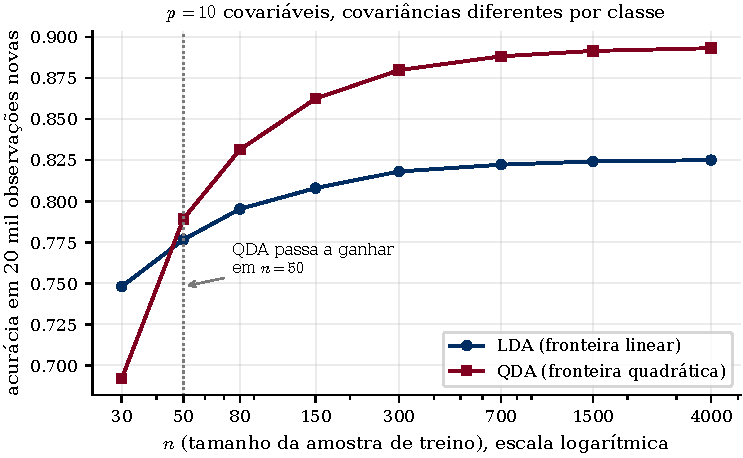
\includegraphics[width=0.72\textwidth]{../../recursos/figuras/07-lda-qda.pdf}
  \caption{Acurácia dos dois métodos em função de $n$, com $p=10$ covariáveis e
  covariâncias genuinamente diferentes por classe --- ou seja, num cenário em que o
  \textbf{QDA está certo e o LDA está errado}. Ainda assim, com $n=30$ o LDA ganha
  ($0{,}748$ contra $0{,}692$): não há dados para estimar $110$ parâmetros de
  covariância, e a variância do QDA supera o viés do LDA. A partir de $n=50$ o jogo
  vira, e em $n=4000$ o QDA abre sete pontos percentuais. Médias de 120 repetições,
  avaliadas em $20\,000$ observações novas.}
  \label{fig:ldaqda}
\end{figure}

\begin{ideia}
Esta figura é a Aula~01 vestida de classificação. O modelo \emph{correto} pode
perder para o modelo \emph{errado} quando não há dados suficientes para estimá-lo
--- exatamente o que o Exemplo~1.7 do [AME] mostrou lá atrás com polinômios de grau
5 e 2. Regra de bolso: LDA com poucas amostras de treino, QDA com muitas ou quando
a hipótese de covariância comum for inverossímil. As duas metades da regra
importam: o que o QDA tem a \emph{perder} depende de $n$ contra os $(K-1)\,p(p+1)/2$
parâmetros que ele estima a mais; o que ele tem a \emph{ganhar} depende de quanto as
covariâncias das classes de fato diferem --- se diferem pouco, não há viés do LDA a
corrigir. E, como sempre, valide de forma cruzada em vez de decidir por regra de
bolso.
\end{ideia}

%==============================================================================
\section{Regressão logística (discriminativo)}
%==============================================================================
O Bayes ingênuo, o LDA e o QDA chegam a $\Prob(Y=c\mid\x)$ por um caminho indireto:
modelam como os dados de cada classe são gerados e invertem com o Teorema de Bayes.
E se estimássemos $\Prob(Y=c\mid\x)$ \emph{diretamente}, sem passar pelas densidades?
É o que fazem os métodos discriminativos, e a regressão logística é o principal
deles. No caso binário $\mathcal{C}=\{0,1\}$ basta modelar $\Prob(Y=1\mid\x)$, com um
cuidado: uma probabilidade vive em $[0,1]$, enquanto uma função linear
$\beta_0+\bbeta^\top\x$ vive em toda a reta. A regressão logística resolve isso
modelando
\begin{equation}\label{eq:logit}
  \Prob(Y=1\mid\x) = \frac{e^{\beta_0+\sum_{i=1}^p\beta_i x_i}}
                          {1+e^{\beta_0+\sum_{i=1}^p\beta_i x_i}}
  = \sigma\big(\beta_0+\bbeta^\top\x\big),
\end{equation}
onde $\sigma(u)=e^u/(1+e^u)$ é a função logística, que leva $\R$ em $(0,1)$.
Equivalentemente, o \emph{log-odds} é linear:
$\log\frac{\Prob(Y=1\mid\x)}{\Prob(Y=0\mid\x)} =\beta_0+\bbeta^\top\x$. Como em
regressão, \emph{não} supomos que isso seja exatamente verdade --- esperamos que
leve a um bom classificador. Note que a fronteira de decisão
$\{\x : \Prob(Y=1\mid\x)=\tfrac12\}$ é o conjunto em que o \emph{log-odds} se anula:
um \textbf{hiperplano}, como no LDA.

\begin{ideia}[por que a logística e não outra curva em $[0,1]$]
A função $\sigma$ tem duas propriedades que a tornam a escolha natural. Primeira:
ela é a inversa do \emph{logit} $\log\frac{p}{1-p}$, que leva $[0,1]$ em toda a reta
--- ou seja, ela transforma um problema restrito num problema linear irrestrito.
Segunda: a linearidade do \emph{log-odds} dá a interpretação que os usuários
querem --- aumentar $x_j$ em uma unidade multiplica a razão de chances por
$e^{\beta_j}$, qualquer que seja o ponto de partida. (O efeito sobre a
\emph{probabilidade}, esse sim, depende de onde se está na curva.) Você vai
reencontrar $\sigma$ na Aula~09 e em qualquer rede neural.
\end{ideia}

\subsection{Estimação por máxima verossimilhança}
Dada uma amostra i.i.d., a verossimilhança condicional é
\begin{equation}\label{eq:vero}
  L(\bbeta) = \prod_{k=1}^n \pi(\x_k)^{Y_k}\big(1-\pi(\x_k)\big)^{1-Y_k},
  \qquad \pi(\x_k)=\Prob(Y_k=1\mid\x_k,\bbeta).
\end{equation}
Maximiza-se o log da verossimilhança \eqref{eq:vero}. Ao contrário do MQO, não há
solução fechada: usam-se métodos numéricos (Newton--Raphson / IRLS). Como na
regressão linear, pode-se \textbf{penalizar} ($\ell_1$/$\ell_2$) para reduzir
variância --- é literalmente a Aula~02 aplicada a outra função-objetivo.

\begin{atencao}[separação perfeita]
Se existir um hiperplano que separa as duas classes \emph{sem erro} no treino, a
verossimilhança \eqref{eq:vero} não tem máximo: empurrar $\norm{\bbeta}\to\infty$
faz as probabilidades tenderem a $0$ e $1$ e a verossimilhança crescer sem parar. O
otimizador roda até o limite de iterações e devolve coeficientes gigantescos e sem
sentido. Acontece com frequência quando $p$ é grande em relação a $n$. A solução é
a penalização --- e é por isso que o \texttt{scikit-learn} aplica $\ell_2$ por
\emph{padrão} na \texttt{LogisticRegression}.
\end{atencao}

\subsection{Mais de duas classes}
Para $\abs{\mathcal{C}}>2$: ou ajusta-se uma logística \emph{um-contra-todos} por
classe (e normaliza-se), ou usa-se a \textbf{regressão logística multinomial}
(\emph{softmax}), que garante que as probabilidades estimadas somem $1$.

%==============================================================================
\section{Discriminativo $\times$ generativo}
%==============================================================================
Com os quatro métodos na mão, vale compará-los. A Figura~\ref{fig:fronteiras} põe as
fronteiras de todos lado a lado, numa mesma amostra de duas classes gaussianas, e a
tabela abaixo resume o que distingue as duas famílias.

\begin{figure}[htbp]
  \centering
  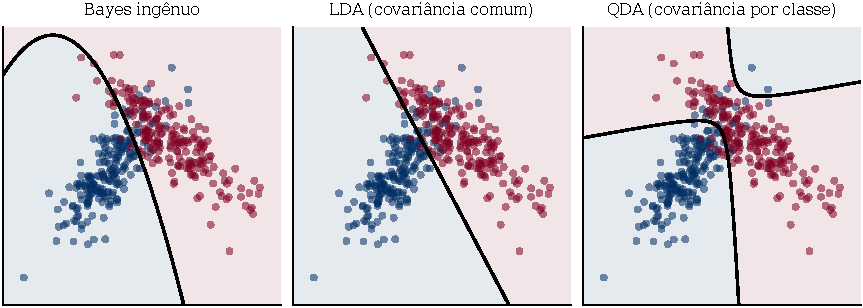
\includegraphics[width=\textwidth]{../../recursos/figuras/07-fronteiras.pdf}
  \caption{Fronteiras de decisão em duas classes gaussianas com covariâncias
  \emph{diferentes} ($n=400$). Logística e LDA chegam a retas quase idênticas por
  caminhos completamente distintos --- uma modelando $\Prob(Y\mid\x)$ direto, a
  outra modelando $f(\x\mid Y)$ e invertendo. O QDA, livre da hipótese de
  covariância comum, curva a fronteira e acompanha o formato de cada nuvem: é o
  modelo correto para estes dados. O Bayes ingênuo também curva, mas erra o ângulo:
  ele supõe as duas covariáveis independentes dentro de cada classe, e aqui elas
  não são.}
  \label{fig:fronteiras}
\end{figure}

\begin{center}\small
\renewcommand{\arraystretch}{1.3}
\begin{tabular}{@{}p{3.2cm}p{5.4cm}p{5.4cm}@{}}
\toprule
 & \textbf{Discriminativo (logística)} & \textbf{Generativo (LDA/QDA/NB)} \\
\midrule
Modela & $\Prob(Y\mid\x)$ direto & $f(\x\mid Y)$ e $\Prob(Y)$ \\
Suposições & poucas (forma do \emph{log-odds}) & distribucionais (gaussiana, indep.) \\
Quando brilha & muitos dados; suposições gaussianas falsas & classes bem separadas; poucos dados; suposições aproximadamente corretas \\
Bônus & --- & gera dados; lida com classes raras \\
\bottomrule
\end{tabular}
\end{center}

\begin{ideia}
Se as suposições gaussianas valem, LDA/QDA são (quase) ótimos e eficientes com
poucos dados. Se não valem, a logística --- que assume menos --- tende a ser mais
robusta com bastante dado. Um detalhe curioso fecha o círculo: sob as hipóteses do
LDA, o \emph{log-odds} sai \textbf{exatamente} linear em $\x$
(Prop.~\ref{prop:lda}), que é justamente o que a logística \eqref{eq:logit} supõe.
Os dois modelos coincidem em forma e diferem só em como estimam os coeficientes ---
o que explica os dois primeiros painéis da Figura~\ref{fig:fronteiras}. Na dúvida:
experimente ambos e compare por validação cruzada.
\end{ideia}

%==============================================================================
\section{Prática em Python}
%==============================================================================
\begin{lstlisting}
from sklearn.naive_bayes import GaussianNB
from sklearn.discriminant_analysis import (LinearDiscriminantAnalysis as LDA,
                                           QuadraticDiscriminantAnalysis as QDA)
from sklearn.linear_model import LogisticRegression
from sklearn.pipeline import make_pipeline
from sklearn.preprocessing import StandardScaler

nb, lda, qda = GaussianNB(), LDA(), QDA()

# Logistica penalizada (C = 1/lambda); padronizar no pipeline (Aula 06)
logit = make_pipeline(StandardScaler(),
                      LogisticRegression(C=1.0, max_iter=1000))

for nome, modelo in [("NB", nb), ("LDA", lda), ("QDA", qda), ("logit", logit)]:
    modelo.fit(X_tr, y_tr)
    print(nome, "acuracia:", modelo.score(X_te, y_te))
    # probabilidades plug-in: modelo.predict_proba(X_te)
\end{lstlisting}

\begin{atencao}
Três pegadinhas. Primeira: em \texttt{LogisticRegression}, o parâmetro é o
\texttt{C}, que é o \textbf{inverso} da penalização --- $C$ \emph{pequeno} significa
regularização \emph{forte}, ao contrário do \texttt{alpha} do Ridge/Lasso.
Segunda: \texttt{modelo.score} devolve \emph{acurácia}, e a caixa de atenção lá do
começo desta aula explica por que isso pode ser uma medida péssima --- leia a
Aula~08 antes de tirar conclusões dessas linhas. Terceira: o \texttt{QDA} das
versões recentes do \texttt{scikit-learn} \emph{recusa} o ajuste quando a
covariância estimada de alguma classe é singular ou quase --- por exemplo, quando a
classe tem no máximo $p$ observações, ou quando há colunas quase colineares. No
segundo caso, o argumento \texttt{reg\_param} puxa as covariâncias levemente na
direção da identidade e resolve (a §8 da \texttt{Aula prática 07} precisa dele);
com menos observações na classe do que covariáveis, nem ele.
\end{atencao}

O notebook \texttt{Comparação entre classificadores paramétricos} põe o Bayes
ingênuo, o LDA e o QDA lado a lado em três conjuntos de dados artificiais, junto com
três SVMs, que são assunto da Aula~09. A \texttt{Aula prática 07} calcula o erro de
Bayes numa população conhecida, compara os quatro métodos desta aula e mede a troca
LDA$\times$QDA em $p=2$ e $p=10$.

%==============================================================================
\section*{Resumo}
%==============================================================================
\begin{itemize}[leftmargin=1.4cm]
  \item Perda 0--1 \eqref{eq:risco01}; o \textbf{classificador de Bayes}
        $g^*(\x)=\argmax_c\Prob(Y=c\mid\x)$ é ótimo (Teo.~\ref{teo:bayes}) mas
        desconhecido --- é a moda condicional, como $r$ era a média condicional.
  \item \emph{Plug-in}: estimar $\Prob(Y=c\mid\x)$ e tomar o $\argmax$ --- ou pelo
        Teorema de Bayes \eqref{eq:gen}, modelando $f(\x\mid Y=c)$ (generativo), ou
        diretamente (discriminativo).
  \item \textbf{Bayes ingênuo}: independência condicional \eqref{eq:nb}, com um
        modelo univariado por covariável (\texttt{GaussianNB},
        \texttt{BernoulliNB}, \texttt{MultinomialNB}, \dots) --- barato, mas
        descalibra quando as covariáveis são correlacionadas.
  \item \textbf{LDA} (covariância comum $\to$ fronteira linear,
        Prop.~\ref{prop:lda}) e \textbf{QDA} (covariância por classe $\to$
        quadrática), com parâmetros por máxima verossimilhança. Ver
        Fig.~\ref{fig:fronteiras}.
  \item LDA $\times$ QDA é viés $\times$ variância (Fig.~\ref{fig:ldaqda}): o
        modelo correto pode perder por falta de dados.
  \item \textbf{Logística} \eqref{eq:logit}: discriminativa, ajustada por máxima
        verossimilhança, penalizável e multiclasse; respeita $[0,1]$ por
        construção, e cuidado com a separação perfeita.
  \item Generativo (eficiente sob suposições corretas e com poucos dados) $\times$
        discriminativo (menos suposições, robusto com muito dado).
  \item Cuidado com acurácia em dados desbalanceados $\Rightarrow$ Aula~08.
\end{itemize}

\paragraph{Leitura recomendada.} [AME] §7.1 (risco 0--1 e o classificador de Bayes,
com o Teorema~9 que é o nosso Teo.~\ref{teo:bayes}), §7.2--7.3 (estimação do risco e
viés--variância em classificação) e §8.1 (a receita \emph{plug-in}, com a logística
em §8.1.2, o Bayes ingênuo em §8.1.3 e a análise discriminante em §8.1.4 ---
atenção: as duas densidades normais escritas ali omitem o $\tfrac12$ do expoente; a
correta é a \eqref{eq:normal}). [ISLP] §2.2.3 (o classificador de Bayes e o erro de
Bayes), §4.3 (a logística, com a interpretação dos coeficientes em razão de chances)
e §4.4 (os modelos generativos: a Figura~4.9 deles é a versão da nossa
Figura~\ref{fig:fronteiras} para LDA e QDA, e o §4.4.3 traz a conta de parâmetros
que está por trás da Figura~\ref{fig:ldaqda}).

\paragraph{Para praticar.} \texttt{Lista teorica 07.pdf} (teórica, com gabarito) e \texttt{Lista prática 07.ipynb} (prática, para completar as lacunas), nesta mesma pasta.

\end{document}
